% rpo.tex
% $Author$ $Date$


        \newif\ifdraft
\drafttrue     % For draft version, commented
%\draftfalse     % For final version, no comments

\ifdraft
    % this style while editing: double spaced, draft
    % \documentclass[draft]{siamltex}     % without figs
    \documentclass{siamltex}          % with figs

\else
    % double spaced, for submission
    % \documentclass[pre,preprint,groupedaddress,showpacs,showkeys]{revtex4}
    % this style for arXiv version, in the journal layout:
    \documentclass[final]{siamltex}
\fi

% \input setup      % PC: not created yet
% \input colordvi
\input defs     % all definitions in defs.tex


                \begin{document}
                \title{
State space geometry of a spatio-temporally chaotic
Kuramoto-Sivashinsky flow
                 }
                  \author{
Predrag Cvitanovi\'c\footnotemark[1],
Ruslan L. Davidchack\footnotemark[2],
    and
Evangelos Siminos\footnotemark[1]
                    }

                \maketitle

\renewcommand{\thefootnote}{\fnsymbol{footnote}}
\footnotetext[1]{
          School of Physics,
          Georgia Institute of Technology, Atlanta, GA 30332-0430, USA
                          }
\footnotetext[2]{
Department of Mathematics, University of Leicester,
            University Road, Leicester LE1 7RH, UK
                }
\renewcommand{\thefootnote}{\arabic{footnote}}

                \begin{abstract}
\PCedit{
The continuous and discrete symmetries of the \KS\ system
restricted to a spatially periodic domain play a prominent
role in shaping the invariant sets of its
spatiotemporally chaotic dynamics.
The continuous spatial
translation symmetry leads to
\reqva\ (traveling wave) and \rpo\ solutions,
with \eqva\ \ES{dropped: and \po s. As we discussed in last skype conference
the \po s do not belong in the antisymmetric subspace (or any other symmetry invariant subspace). The initial point $u(x,0)$
and mid-point $u(x,T_p/2)$ are related by $\Refl\Shift_{\shift_p/L} u(x,\period{p}/2) = 
-u(-x-\shift_p,\period{p}/2) = u(x,0)$ but the profile $u_p(x)$ of the \po\ does not lie in a symmetry restricted subspace
at any instant.}  restricted to the discrete reflection symmetry
subspaces.  The discrete symmetries induce decomposition
of phase space into orthogonal invariant subspaces and allow for the
existence of structurally stable heteroclinic connections between \eqva.
We show, on example of a particular small-cell \KS\ system,
how the geometry of its dynamical \statesp\ is organized by a rigid
`cage' built by heteroclinic connections between \eqva, %and \rpo s,
and demonstrate the preponderance of unstable \rpo s and their likely
role as the skeleton underpinning spatiotemporal turbulence in systems
with continuous symmetries.
Presence of
continuous symmetries makes a visualization of high-dimensional
\statesp\ flows
not straightforward.  We introduce novel visualizations of the \KS\ flow
through projections onto low-dimensional
dynamically invariant frames,
as well as in terms of physical, symmetry invariant observables.
       }
                \end{abstract}

\begin{keywords}
relative periodic orbits, chaos, turbulence, continuous symmetry, {\KSe}
\end{keywords}

\begin{AMS}
35B05, 35B10, 37L05, 37L20, 76F20, 65H10, 90C53
\end{AMS}

\pagestyle{myheadings}
\thispagestyle{plain}
\markboth{P.~CVITANOVI\'C, R.~L. DAVIDCHACK, AND E.~SIMINOS}
         {GEOMETRY OF A CHAOTIC KURAMOTO-SIVASHINSKY FLOW}

% siminos/kittens/intro.tex      pdflatex CL18
% $Author: predrag $ $Date: 2020-08-02 22:02:31 -0500 (Sun, 02 Aug 2020) $


\section{Introduction}
\label{s:intro}

A temporally chaotic system is exponentially unstable with time: double the
time, and exponentially more \po s are required to cover its strange
attractor to the same accuracy. For large spatial extents, the complexity of
the spatial shapes also needs to be taken into account; double the spatial
extent in a given direction, and exponentially as many distinct
{\spt} patterns will be required to describe the repertoire of
system's shapes to the same accuracy.
The systems whose temporal and spatial correlations decay sufficiently fast,
and whose ``physical'' dimension\rf{ginelli-2007-99,DCTSCD14} grows with
system size, are said to be ``{\spt}ly chaotic.''

    \PC{2019-12-27}{
\catlatt\ = classical field theory on a $d$\dmn\ hyper-cubic lattice, with an
``anti-harmonic" rotor at each site, coupled to its nearest neighbors
    }

    \PC{2019-06-26}{
Physical picture:

Turbulence everywhere in space, with a range of length scales. Discretize into
cells, with each cell turbulent, and cells coupled
to their nearest neighbors\rf{Kaneko83}.

As a function of the strengths of cell-cell couplings, dynamics can exhibit rich
phase-transitions structure\rf{Kaneko84}. In this paper we chose couplings such
that the system is fully turbulent.

Explain word ``turbulence" as used here.

Hamiltonan, so symplectic or area preserving, but that is not essential.
Cite the Hamiltonian zeta function
from ChaosBook.

The main point: we've been doing it all wrong, and we know that since
\Poincare.
In ``explaining'' chaos we talk the talk as though we never moved beyond Newton.
But people who actually compute solutions do something altogether different,
closer to Lagrange (and the late 20th century, `spacetime' physics).
This paper realigns the theory to what we actually {\em do} when
solving ``chaos'' equations, using nothing more than the well known linear
algebra.
    }

coupled map lattice models

the spacetime discretized

dynamics of small-scale spatial structures modeled by discrete time
maps

single cell dynamics  attached to lattice sites,

coupling to neighboring sites

the Gutkin and Osipov\rf{GutOsi15}
$d$\dmn\ coupled cat maps lattice
(``{\catlatt}'' for short, in what follows),
a {\spt} generalization of the Percival and Vivaldi\rf{PerViv} {linear
code} for temporal evolution of a single cat map


the $d$\dmn\ lattice {\sPe}
\[
 (\Box -s+2d)\,\ssp_{z}  =  -\Ssym{z}
 \,.
\]

from the cat maps (modeling the
Hamiltonian dynamics of individual ``particles'') at sites of a
$(d\!-\!1)$\dmn\ spatial lattice, linearly coupled to their nearest
neighbors.

solution $\Xx$ of a global fixed-point condition
$F[\Xx]=0$ is uniquely encoded by a finite alphabet $d$\dmn\ symbol
lattice state  $\Mm$



which symbol \brick s are {\admissible}?

The  linearity of the {\catlatt} enables us to

standard crystallographic  methods\rf{Dresselhaus07} and
integer lattices counting\rf{Barvinok08} enable us to count {\spt}ly finite \brick s,
and give explicit formulas for the number of \dtor\ solutions
for \brick s of any size.

Implementing this program requires several tools not standard in
dynamicist's tool box: lattice Green's functions; lattice determinants.

We start the paper with a reformulation of the 1 degree of freedom
Bernoulli map, because our goal, the \catlatt\ is nothing but its
generalization to a mechanical system in spacetimes of arbitrary
dimension, and thus arguably the simplest possible example of a `chaotic
field theory'.

\bigskip

The paper is organized as follows:
For a reader too busy\rf{focusPOT} to read the book\rf{ChaosBook}, we
start in \refsect{s:coinToss} with a brief course on `chaos' theory,
disguised as a humble coin toss. The deep insight here is the realization
that the volume \refeq{detBern0} of the {\jacobianOrb} (the functional
determinant of the {\fundPip} or the {\HillDet}, see
\reffig{fig:BernCyc2Jacob}, \ref{fig:catCycJacob} and
\ref{fig:BravaisLatt}), counts the numbers of global solutions for a
given `law', true at all times and at all spatial positions.
Before turning to the spatially infinite field theory in
\refsect{s:catlatt}, it is instructive to motivate our formulation of the
{\catlatt} by investigating the temporal lattice Bernoulli and cat
systems (\ie, `\spt\ lattices' with only one site in the spatial
direction).
In \refsect{s:catPV} we review the traditional cat map in its usual,
Hamiltonian formulation,  and \refappe{s:catMapHam} construct an explicit
generating (\AW) partition of the cat map \statesp.
In \refsect{s:catLagrange} we introduce the `\templatt', a global lattice
reformulation of the cat map.
The \po s theory of cat maps, \refsect{s:tempCatCount}, can be developed in either
formulation:
both the Hamiltonian cat map \po s counting (\refappe{s:catHamCount}) and
the Lagrangian {\templatt} \po s counting (\refsect{s:tempCatCount}) lead
to the same {\tzeta}, with the two formulations related by {Hill's
formula} (\refsect{s:HillForm}).
A reader may skip \refSecttosect{s:catPV}{s:tempCatCount} on the
first reading, as the paper proper starts with \refsect{s:catlatt}.

In \refsect{s:catlatt} (after a brief review of the traditional coupled
map lattices, \refsect{s:CCMs}), we extend the \templatt\ to
the $d$\dmn\ \catlatt, \refsect{s:dDcatLatt}.
In \refsect{s:BravaisLatt} we show that the system admits  a natural
$d$\dmn\ symbolic  code with a finite alphabet, and then study finite
{\spt} symbol \brick s.

\refSect{s:catLattCount} %~{\em Invariant tori in $d$\dmn\ \catlatt}
describes our counting solutions of a
$d$\dmn\ \catlatt.

In \refsect{s:catLattShadow}  we use these  results to construct
sets of {\spt} \twots\ that partially shadow each other.

The results are summarized and some open questions discussed in the
\refsect{s:summary}.

In \refappe{s-SymbDynGloss} we collect the symbolic dynamics definitions
needed throughout the paper.

% KSe.tex
% $Author$ $Date$

% \section{\KSe}
% \label{s-KS}
% Predrag                    4jul2006
% Predrag                   jun 20 2006
% Vaggelis                  may 20 2006
% extracted from ~dasbuch/book/chapter/PDEs.tex  5jun2005 version
% Predrag                   17sep1999

% \PC{incorporate missing refs from chapter/refsPDEs.tex}

The \KS\ [henceforth KS] system\rf{ku,siv},
which arises in the description of
stability of flame fronts, reaction-diffusion systems and many other
physical settings\rf{KNSks90}, is one of the simplest nonlinear PDEs that
exhibit spatiotemporally chaotic behavior. In the formulation
adopted here, the time evolution of the `flame front velocity'
$u=u(x,t)$ on a periodic domain $u(x,t) = u(x+L,t)$ is given by
\beq
  u_t+{\textstyle\frac{1}{2}}(u^2)_x+u_{xx}+ u_{xxxx}=0
% abandoned the CCP convention: u_t=(u^2)_x-u_{xx}- u_{xxxx}
    \,,\qquad   x \in [-L/2,L/2]
    \,.
\ee{ks}
Here $t \geq 0$ is the time, and $x$ is the spatial coordinate.
The subscripts $x$ and $t$ denote partial derivatives with respect to
$x$ and $t$.
% In the literature \refeq{ks} is sometimes written as
% \[ %beq
%     u_t=(u^2)_x-u_{xx}- \nu \, u_{xxxx}
%     \,,\qquad   x \in [0,L]
%     \,,
% \] %\ee{ksVisc}
% or in any number of other variants, all equivalent.
In what follows
we shall state results of all calculations either in units of the
`dimensionless system size' $\tildeL$, or the system size $L = 2 \pi
\tildeL$. %, with the `hyper-viscosity' $\nu$ fixed to $1$. Other
% authors vary  $\nu$, with $L$ fixed to either $1$ or $2\pi$.
All numerical results presented in this paper
are for the system size $\tildeL=22/2\pi = 3.5014\cdots$.
Spatial periodicity $u(x,t)=u(x+L,t)$
makes it convenient to work in the Fourier space,
\beq
  u(x,t)=\sum_{k=-\infty}^{+\infty} a_k (t) e^{ i k x /\tildeL }
\,,
% \label{fseries}
\ee{eq:ksexp}
%where $\tildeL=L/2\pi$. Thus,
with the $1$-dimensional PDE \refeq{ks}
replaced by an infinite set of
ODEs for the complex Fourier coefficients $a_k(t)$:
\beq
\dot{a}_k= \pVeloc_k(a)
     = ( (k/\tildeL)^2 - ( k/\tildeL)^4 )\, a_k
    - i \frac{k}{2\tildeL} \sum_{m=-\infty}^{+\infty} a_m a_{k-m}
\,.
\ee{expan}
Since $u(x,t)$ is real, $a_k=a_{-k}^\ast$, and we can replace the
sum by a $k > 0$ sum.

\PC{find better place for this text?}
Due to the hyperviscous damping $u_{xxxx}$, long time solutions of
\KSe\ are smooth, $a_k$ drop off fast\PC{how fast?} with $k$,
and truncations of \refeq{expan} to $16 \leq d \leq 128$  terms
yield accurate solutions for system sizes considered here.
Robustness of the long-time dynamics of KS as a function of the
number of Fourier modes kept in truncations of \refeq{expan} is, however,
a subtle issue.
Adding an extra mode to a truncation of the system
introduces a small perturbation in the space of dynamical
systems. However, due to the lack
of structural stability both as a function of truncation $d$, and the
system size \tildeL, a small variation in a system parameter
can (and often will) throw the dynamics
into a different asymptotic state.
For example, asymptotic attractor
which appears to be chaotic in a $d$-dimensional
\statesp\ truncation can
collapse into an attractive period-$n$ cycle for
$(d\!+\!1)$-dimensions.

%%%%%%%%%%%%%%%%%%%%%%%%%%%%%%%%%%%%%%%%%%%%%%%%%%%%%%%%%%%%%%
\begin{figure}[t]
\begin{center}
%\includegraphics[width=0.8\textwidth]{figs/ks_largeL.eps}
\includegraphics[width=0.9\textwidth]{figs/ks_largeL_cbar.eps}
\end{center}
\caption{
A typical `turbulent' solution of the \KSe, system size
$L=20\pi\sqrt{2}\approx 88.86$.  The $x$ coordinate is scaled
with the most unstable wavelength $2\pi\sqrt{2}$, which is
approximately also the mean wavelength of the turbulent flow.
The color bar indicates the color scheme for $u(x,t)$.  This color
scheme is used in other figures of this type throughout this work.
     } \label{f:ks_largeL}
\end{figure}
%%%%%%%%%%%%%%%%%%%%%%%%%%%%%%%%%%%%%%%%%%%%%%%%%%%%%%%%%%%%%%%%%%

\subsection{Symmetries of \KSe}
\label{sec:KSeSymm}

The KS equation is Galilean invariant: if $u(x,t)$ is a solution,
then $u(x \PCedit{-ct,t) -c} $, with $c$ an arbitrary constant
speed, is also a solution. Without loss of generality, in our
calculations we shall set the mean velocity of the front to zero,
\beq \int dx \, u = 0 \,. \ee{GalInv}
As $\dot{a_0}=0$ in
\refeq{expan}, $a_0$ is a conserved quantity, in our calculations
fixed to $a_0=0$ by the
% Galilean invariance
condition \refeq{GalInv}.
$G$, the group of actions $ g \in G $
on a \statesp\ (reflections, \PCedit{translations}, \etc)
is a symmetry of the flow
$\dot{u} = F(u)$ if $g\,\dot{u} = F(g\,u)$.
The KS equation % \refeq{ks}, 
\beq
\dot{u} = 
F(u) = -u u_x-u_{xx}- u_{xxxx}
% \,,
\ee{KSO2}
is time
translationally invariant, and space translationally invariant
on a periodic domain under
the 1-parameter group of 
\PCedit{
$O(2): \{\Shift_{\shift/L},\Refl \}$.
       }
If $u(x,t)$ is a solution, then
$\Shift_{\shift/L}\, u(x) = u(x+\shift,t)$
is an equivalent solution for any \PCedit{shift}
$-L/2 < \shift \leq L/2$,
as is the
reflection (`parity' or `inversion')
\beq
    \Refl \, u(x) = -u(-x)
\,.
\ee{KSparity}
The translation operator action on the Fourier coefficients
\beq
  (\Shift_{\shift/L}\, a)_k= e^{ik\, \shift /\tildeL} \, a_k
    \qquad \mbox{(no summation on $k$)}
    \,.
    \label{eq:RPOcondFouri}
\eeq
amounts to the $k$-th mode complex plane rotation by an angle
$-k\, \shift /\tildeL$, and the reflections acts on them
by complex conjugation,
\beq
  \Refl \, a_k = -a_k^\ast
% a_{2m} \to a_{2m}
\,.
\ee{FModInvSymm}
Reflection generates the dihedral subgroup $D_1 = \{1, \Refl\}$ 
of $O(2)$.  Let $\bbU$ be the space of
real-valued velocity fields periodic and square integrable
on the interval $\Omega = [-L/2,L/2]$,
\begin{align}
 \bbU  &= \{u \in L^2(\Omega) \; | \; u(x) = u(x+L)\}  \,.
\end{align}
A continuous symmetry maps each state $u \in \bbU$ 
to a manifold of functions with identical dynamic behavior.
Relation $\Refl^2 = 1$ induces linear decomposition
$u(x) = u^+(x)+ u^-(x)$, 
\PCedit{
$u^\pm(x)= P^\pm u(x) \in  \bbU^\pm$,
into irreducible subspaces
$
\bbU = \bbU^+  % \oplus  \bbUsymm
       \oplus \bbU^-
$, where
        }
\beq
    P^+=(\matId+\Refl)/2
    \,,\qquad
    P^-=(\matId-\Refl)/2
\ee{P1P2proj}
are the antisymmetric/symmetric projection operators.
Applying $P^+,\,P^-$ on the KS equation \refeq{KSO2}
we have\rf{KNSks90}
\bea
 u_t^+ &=& - (u^+u^+_x + u^-u^-_x )
                - u^+_{xx} - u^+_{xxxx}
    \continue
 u_t^- &=& - (u^+u^-_x + u^-u^+_x )
                - u^-_{xx} - u^-_{xxxx}
\,.
\label{KSD1}
\eea
If $u^- = 0$, KS flow is confined to
the antisymmetric $\bbU^+$ subspace,
\beq
 u_t^+ = - u^+u^+_x
                - u^+_{xx} - u^+_{xxxx}
%        \,,\qquad   x \in
\,,
\label{KSU+}
\eeq
but otherwise the nonlinear terms in \refeq{KSD1}
mix the two subspaces.
    \PC{still to be incorporated, most likely in the next paper:
    wrote down \refeq{KSD1} in order to (a) to clarify embedding of
    $\bbU^+$ into $\bbU$
    (b) to explain the desymmetrization of evolution defined on
     $\Omega^{+} = [0, L/2]$ fundamental domain, with evolution at
    instant of crossing $x=0$ given by reflection $\Refl$.
    Re integrators: make sure $\Refl$ applied after
    all points used by integrator are in $\bbU^-$
    }


Together with any rational shift
$ \Shift_{1/m}u(x)=u(x+L/m)$
reflection generates a discrete dihedral $D_m$
subgroup of $O(2)$, also a symmetry of KS.
The only non-zero Fourier components of a solution invariant
under $D_m$ are $a_{jm} \neq 0$, $j =1,2,\cdots$ .
$D_m$ reduces the dimensionality
of \statesp\ and aids computation of \eqva\ and \po s
within it. For example, the 1/2-cell translations 
\ES{moved all references to 1/2-cell translation to one place.}
\beq
    \Shift_{1/2}\, u(x)=u(x+L/2)
\,,
\ee{KSshift}
and reflections generate $O(2)$
subgroup $D_2 = \{1, \Refl,\Shift,\Shift\Refl\}$,
which
reduces the \statesp\ into four irreducible subspaces
(for brevity, here $\Shift = \Shift_{1/2}$):
\PC{dangerous edit, changed $S \to A$ for reflections,
    please cross-check}
\PCedit{
\begin{align}
 & \qquad\qquad\qquad\qquad\qquad
              ~~~ \Shift ~~ \Refl  ~\;  \Shift\Refl
    \nnu\\
P^{(1)} &= \frac{1}{4} (1 + \Shift + \Refl + \Shift\Refl)
           ~~~~  S  ~~  A   ~~   A
    \nnu\\
P^{(2)} &= \frac{1}{4} (1 + \Shift - \Refl - \Shift\Refl)
            ~~~~  S  ~~  S   ~~   S
    \nnu\\
P^{(3)} &= \frac{1}{4} (1 - \Shift + \Refl - \Shift\Refl)
           ~~~~  A  ~~  A   ~~   S
     \label{ek_defn}\\
P^{(4)} &= \frac{1}{4} (1 - \Shift - \Refl + \Shift\Refl)
          ~~~~  A  ~~  S   ~~   A
\,.
    \nnu
\end{align}
        }
$P^{(j)}$ is the projection operator onto
$u^{(j)}$ irreducible subspace, and the last 3 columns
refer to the symmetry of
$u^{(j)}$ functions under reflection and
1/2-cell shift.
By the same argument that identified \refeq{KSU+} as
the invariant subspace of KS, here the KS flow
stays within the  
\PCedit{
 $\bbU^S =  \bbU^{(1)}+ \bbU^{(2)}$ 
irreducible $D_1$ subspace of $\bbU$
       } 
profiles symmetric under 1/2-cell shifts.

    \PC{abandoned the \refref{KNSks90} notation, I might be wrong,
        please recheck. Replace $\mathbf{L} \to P^{(1)}$ downstream}
\PCedit{
While in general the bilinear term $(u^2)_x$  mixes the
irreducible subspaces of $D_n$, for $D_2$ there are
four subspaces invariant under the flow\rf{KNSks90}:
\begin{romannum} % SIAM itemize}
 \item[$\{0\}$:~~~~~~] the $u(x)=0$ {\eqv}
 \item[$\bbU^+ = \bbU^{(1)}+ \bbU^{(3)} $:] 
    the reflection $D_1$ irreducible space of antisymmetric $u(x)$
 \item[$\bbU^S =  \bbU^{(1)}+ \bbU^{(2)}$:] 
    the shift $D_1$ irreducible space of $L/2$ shift symmetric  $u(x)$
 \item[$\bbU^{(1)}$:~~~~~]
    the $D_2$ irreducible  space of $u(x)$ invariant under $x\mapsto L/2-x,\ u\mapsto -u$
\end{romannum} %itemize}
as long as all other components of $u(x)$ are 
set to zero (see for example \refeq{KSU+}).
        } % end \PCedit
With the continuous
translational symmetry eliminated within each subspace, there are no
\reqva\ and \rpo s, and one
can focus on the \eqva\ and \po s only, as was done
for $\bbU^+$ in \refrefs{Christiansen:97,Lan:Thesis,LanCvi07}.
In the Fourier
representation, the 
\PCedit{
$u \in \bbU^+$
    }
antisymmetry amounts to having purely imaginary
coefficients, since $a_{-k}= a^\ast_k = -a_k$.
The 1/2 cell-size shift $\Shift_{1/2}$
generated 2-element discrete subgroup
$\{1,\Shift_{1/2}\}$ is
of particular interest
because in the 
\PCedit{
$\bbU^+$
       }
subspace the translational invariance of the full system reduces to
invariance under discrete translation \refeq{KSshift} by half a
spatial period $L/2$.

Each of the above dynamically invariant subspaces is unstable
under small perturbations, and generic solutions of \KSe\ belong to
the full space.
Nevertheless, since  all \eqva\ of the KS flow studied in this paper
lie in the $\bbU^+$ subspace (see
\refsect{sec:L22}), $\bbU^+$  plays important role for the global
geometry of the flow.
However, linearized stability of these \eqva\ has
eigenvectors both in and outside of $\bbU^+$, and needs to be
computed in the full \statesp.
% via four products $\Refl_{1,2} \Shift_{1,2}$



\subsection{\Eqva\ and \reqva} % of the \KSe}
\label{sec:stks}
% former equilibria.tex

% Predrag                   jun 20 2006
% Vaggelis                  may 20 2006
% Predrag                                       05dec2004
% Lan                                           25nov2004
% from Lan thesis                                8jun2004

\Eqva\  (or the steady solutions)
are the fixed profile time-invariant solutions,
\beq
 u(x,t) = u_\stagn(x) %\,,\quad t \in \mathbb{R}
\,.
\ee{eqva}
Due to the translational symmetry,
the KS system also allows for 
\reqva\ (traveling waves, rotating waves),
characterized by a fixed profile $u_\stagn(x)$
moving with constant speed $c$, {\ie}
\beq
 u(x,t) =  u_\stagn(x-ct) %\,,\quad t \in \mathbb{R}
\,.
\ee{reqva}
Here suffix ${}_\stagn$ labels a particular invariant solution.
Because of the reflection symmetry \refeq{KSparity},
the \reqva\ come in counter-traveling pairs
$u_\stagn(x-ct)$, $-u_\stagn(-x+ct)$.

The \reqv\ condition for the {\KS} PDE \refeq{ks}
is the ODE
\beq
{\textstyle\frac{1}{2}}(u^2)_x+u_{xx}+ u_{xxxx}=c \, u_x
% \,.
\ee{KSeqvCond}
which can be analyzed as a dynamical system in its own right.
\PC{\PCedit{PC: please recheck $E$ vs $c$}}
Integrating once we get
\PC{
    \reqva\ = \eqva\ shifted by $c$?
   }
\ESedit{
\beq
{\textstyle\frac{1}{2}}u^2 - c u + u_x + u_{xxx}=\expctE
\,.
\label{eq:stdks}
\eeq
}%End ESedit
This equation can be interpreted as a 3-dimen\-si\-on\-al dynamical system
with spatial coordinate $x$ playing the role of `time' and integration constant \expctE\ can be interpreted as `energy',
see \refsect{sec:energy}.
% Integrate over $L$, and $u_x$, $u_{xx}$ drop put by the
%  $L$ periodicity.
% Written as a ,
%\refeq{eq:stdks}
% this is a volume preserving flow
% % \beq
% % \ESedit{
% % v = u_x \,,\qquad
% % w = v_x \,,\qquad
% % w_x = \expctE - {\textstyle\frac{1}{2}} u^2 + c u - v 
% %        }% end ESedit
% % \,,
%   \label{eq:3dks}
% \eeq
% \ES{
% Changed signs here, seemed simpler this way. 
% PC: I remember having a reason, so something down the line 
%     came out with consistent signs. Perhaps \refeq{eqvOfEqv}?
%    }
% with the `time' reversal symmetry,
% \[
% x \to -x,\quad u \to -u, \quad v \to v, \quad w \to -w \,.
% \]
%     \ES{
%    The term $c u$ breaks the symmetry. 
%    We may overcome this by changing sign of c as well, 
%    but it is a parameter, not a variable.
%        }
% \PC{might move space average def \refeq{rpo:spac_ave} to here,
%     note that
%     $\expct{u} = \expct{v} = \expct{w} =0$
%     }
%  Rewriting \refeq{eq:3dks} as 
%      \ES{With the corrected form of \refeq{eq:stdks} we cannot write this}
% \beq
% \PCedit{
% (u+w)_x={\textstyle\frac{1}{2}}(u-c)^2-\expctE
%     ={\textstyle\frac{1}{2}}(u-c-\sqrt{2\expctE}) (u-c+\sqrt{2\expctE})
%        } %end \PCedit{
% \ee{eqvOfEqv}
% we see that
% for $\expctE<0$, 
%     \ES{Isn't $E>0$ by definition?
%     PC: Here $E$ is an integration constant - do not see how
%     we can argue $E \geq 0$ at this point.
%         } 
% $u+w$ increases without bound with $x \to \infty$,
% and every solution escapes to infinity.
% If $\expctE=0$, the origin $(0,0,0)$ is the
% only bounded  solution, a marginally stable center with
% eigenvalues $(0, i,-i)$.

For $\expctE>0$ there is rich
$\expctE$-dependent dynamics, with
fractal sets of bounded solutions investigated in
depth by Michelson\rf{Mks86}.
%
% former\subsection{Bifurcation structure of \eqva\ and \reqva.}
% \label{sec:KSlit}
% Vaggelis               jan 20 2007
%
For $\tildeL<1$ the only \eqv\ of the system is the
globally attracting constant
solution $u(x,t)=0$, denoted $\EQV{0}$ from now on. With increasing system size $L$ system
undergoes a series of bifurcations.
The resulting \eqva\ and
\reqva\ (but not \po s and \rpo s)
are described in the classical papers of
Kevrekidis, Nicolaenko and Scovel\rf{KNSks90},
and Greene and Kim\rf{ksgreene88},
The relevant bifurcations
up to the system size
investigated here are summarized
in \reffig{fig:ksBifDiag}:
at $\tildeL=22/2\pi =
3.5014\cdots$, the {\eqva} are the constant solution
\EQV{0}, the GLMRT\rf{laquey74,ksgreene88} \eqv\ \EQV{1}, the $2$-
and $3$-cell states \EQV{2} and \EQV{3}, the pair of \reqva\
\REQV{\pm}{1}, and the  \REQV{\pm}{2} \reqva.

%%%%%%%%%%%%%%%%%%%%%%%%%%%%%%%%%%%%%%%%%%%%%%%%%%%%%%%%%%%%%%%%
\begin{figure}[t]       \label{fig:ksBifDiag}
\begin{center}
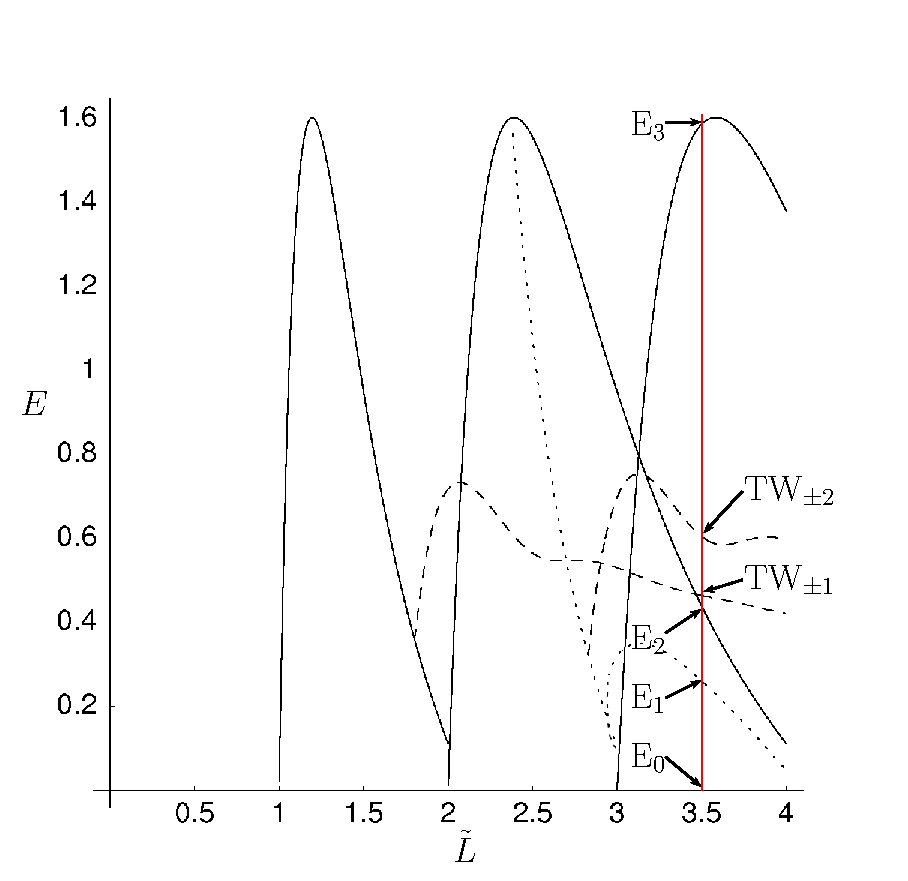
\includegraphics[width=0.5\textwidth]{figs/ksBifDiag_pst.eps}
\end{center}
\caption{
The energy \refeq{ksEnergy} of the \eqva\ and \reqva\ that
exist up to $L=22$, $\tildeL = 3.5014\cdots$, plotted as a function
of the system size $\tildeL = L/2\pi$ (additional \eqva, not present
at $L = 22$ are given in \refref{ksgreene88}). Solid curves denote
$n$-cell solutions \EQV{2} and \EQV{3}, dotted curves the GLMRT
\eqv\ \EQV{1},
% the dash-dotted curve the `giant states' (??? don't have those),
and dashed curves the \reqva\ \REQV{\pm}{1} and \REQV{\pm}{2}.
The parameter $\alpha$ of \refrefs{KNSks90,ksgreene88} is
related to the system size by $\tildeL=\sqrt{\alpha/4}$.
% Open circles indicate Hopf bifurcations.
%The color of a branch indicates the number of unstable eigenvalues:
%(red) 2 unstable eigenvalues, (blue) 1 unstable eigenvalue, (green)
%stable.
        }
\end{figure}
%%%%%%%%%%%%%%%%%%%%%%%%%%%%%%%%%%%%%%%%%%%%%%%%%%%%%%%%%%%%%%%%%%

\ES{Removed text about equilibria of equilibria.}
% ES removed
%%%%%%%%%%%%%%%%%%%%%%%%%%%%%%%%%%%%%%%%%%%%%%%%%%%%%%5
% The solutions of the {\eqv}  condition
% \refeq{eq:3dks} are
% % themselves in turn
% organized\rf{Mks86} by the
% `{\eqva}  of {\eqva}'  condition
% \( u_x= v_x= w_x= 0 \).
% % , and the connections between them.
%     For $\expctE>0$ the {\reqva}  points of \refeq{eqvOfEqv} are
% $C_{+}=(c+\sqrt{2\expctE},0,0)$ and $C_{-}=(c-\sqrt{2\expctE},0,0)$.
% Linearization of the flow around $C_{+}$ yields the cubic equation
% $ %  \beq
% \eigExp(1+\eigExp^2) = 4 \expctE
% \,,
% $ %  \ee{KSeqvCubic}
% with linear stability eigenvalues
% \beq
% \eigExp[1] = 2 \eigRe
%     \,,\qquad
% \eigExp[2,3] = - \eigRe \pm i \eigIm
% \ee{eqvEqvEigV}
% Hence $C_{+}$ has a {1\dmn}
% unstable manifold and a 2\dmn\ stable manifold
% along which solutions spiral in.
% By the $x \to -x$ `time reversal' symmetry, the
% invariant manifolds of $C_{-}$
% have reversed stability properties.
% \PC{
%     not sure we need this, not used in our paper? Where did the figure go?
%     }
% Most orbits escape quickly even if initiated close to \eqva, and that
% renders the numerical calculations
% difficult\rf{ksham95,kshooper88,pimyk,pimsimp}.
% In this context the variational method
% developed in \refrefs{lanVar1,CvitLanCrete02}
% appears more robust than
% the earlier approaches.
%%%%%%%%%%%%%%%%%%%%%%%%%%%%%%%%%%
% end ES removed

%\subsection{\Eqva\ on a periodic domain}
%

%\RLD{This paragraph should probably be moved down after real-space
%equation for equilibria and traveling waves are discussed.}
In the Fourier representation the \reqva\ time
dependence is
\beq
 a_k(t) e^{-itc k/\tildeL} = a_k(0)
\,.
\ee{reqvaF}
Differentiating with respect to time, we obtain
the Fourier space version of the \reqv\ condition
\beq
 \pVeloc_k(a) - i \frac{k c}{\tildeL} a_k = 0
\,,
\ee{reqvCondF}
which we solve for (time independent) $a_k$ and $c$.
Periods of spatially periodic {\eqva} are multiples of $L$.
Every time the system size crosses  $\tildeL=n$,
$n$-cell states
are generated through pitchfork bifurcations off $u =0$
equilibrium.
Due to the translational invariance of {\KSe},
they form invariant circles
in the full \statesp.
In the $\bbU^+$ subspace considered here,
they correspond to $2n$ points, each shifted by $L/2n$.
For a sufficiently small $L$
the number of {\eqva} is small and
concentrated on the low wave-number end of the Fourier spectrum.

In a periodic box of size $L$
both \eqva\ and \reqva\ are  periodic solutions
embedded in 3-$d$ space,
conveniently represented as loops in
$(u,u_x,u_{xx})$ space \ES{dropped 
whose topology is controlled by the
`\eqva\ of \eqva' stable-unstable manifold structure of
\refeq{eqvEqvEigV} }
, see \reffig{f:KS22Equil}\,(\textit{d}).
In this representation the continuous translation symmetry
is automatic - a rotation in the $[0,L]$ periodic domain only
moves the points along the loop. For an \eqv\ the points
are stationary in time; for \reqv\ they move in time, but in
either case, the loop remains invariant.
So we do not have the problem that we encounter in the Fourier
representation, where from the frame of one of the \eqva\
the rest trace out circles under the action of continuous symmetry
translations.


\subsection{Stability of \eqva}
\label{s:StabEqui}
%%
% Predrag           5jun2005
% extracted from \Chapter{stability}{ 2apr2005}

If $u_\stagn(x)$ is an \eqv\ solution of \KSe,
the {\stabmat}
${\Mvar}={\Mvar}(a_\stagn)$
is constant in time,
and
the {\jacobianM}
of the \eqv\ solution is
\beq
 \jMps^t(a_\stagn) = e^{{\Mvar} t}
    \,,\qquad
 \Mvar_{ij}= \Mvar_{ij}(a_\stagn)
\,.
\ee{eqvFundMat}
Calculation of the {\stabmat} requires a bit of care:
% \refeq{DerMatrix}
$a_{k}$ cannot be varied independently of $a_{-k}$, as
% \refeq{expan}
the reality of $u(x,t)$ implies that $a_{k}=a^*_{-k}$.
We impose the reality constraint by splitting \refeq{expan}
in real and imaginary parts, $a_k=b_k+i\, c_k$. {\Stabmat}
is then:
% \index{Kuramoto-Sivashinsky system}
\bea
    \frac{\partial \dot{c}_k}{\partial c_{j}} & = &
    \frac{k^2}{\tildeL^2}\left(1- \frac{k^2}{\tildeL^2} \right)\delta_{kj}
    - \frac{k}{\tildeL} (c_{k+j}-c_{k-j})
\continue
    \frac{\partial \dot{c}_k}{\partial b_{j}} & = &
    - \frac{k}{\tildeL} ( b_{k+j}+b_{k-j} )
\label{expanMvar}\\
    \frac{\partial \dot{b}_k}{\partial b_{j}} & = &
    \frac{k^2}{\tildeL^2}\left(1- \frac{k^2}{\tildeL^2} \right)\delta_{kj}
    +  \frac{k}{\tildeL} (c_{k+j} + c_{k-j})
\continue
    \frac{\partial \dot{b}_k}{\partial c_{j}} & = &
    - \frac{k}{\tildeL} (b_{k+j}-b_{k-j})
    \,,\qquad  k,j>0
\,.
\nnu
\eea
For the \KSe\ the constant solution $u(x,t)=0$ with zero energy $E$ is an
\eqv\ point of \refeq{ks} which we shall henceforth refer to as
\EQV{0}. For this `laminar' \eqv\ the {\stabmat}
is diagonal, and
so is the {\jacobianM}
$
\jMps^t_{kj}(0) = \delta_{kj} e^{(k/\tildeL)^2(1- (k/\tildeL)^2)t}
\,.
$

From \refeq{expan} we see that the origin $u(x,t) = 0$
has Fourier modes as the linear stability eigenvectors.
The $|k|<\tildeL$
long wavelength perturbations of the flat-front {\eqv}
are linearly unstable, while all
$|k|> \tildeL$ short wavelength perturbations are strongly contractive.
The high $k$ eigenvalues, corresponding to rapid variations of
the flame front, decay so fast that the corresponding eigendirections
are physically irrelevant.
The most unstable mode, nearest to $|k|=\tildeL/\sqrt{2}$,
sets the scale of the mean wavelength $\sqrt{2}$
of the KS `turbulent' dynamics,
% measured in the system size \tildeL,
see \reffig{f:ks_largeL}.

\subsection{\Rpo s, symmetries and \po s} \label{sec:KSePO}
% Predrag created file              jul 3 2006

The KS equation \refeq{ks} is time translationally invariant,
and space translationally invariant
under the 1-$d$ Lie group of $O(2)$ rotations: if
$u(x,t)$ is a solution, then $u(x+\shift,t)$ and
$-u(-x+\shift,t)$ are equivalent
solutions for any $-L/2 < \shift \leq L/2$.
As a result, KS can have
%\reqva\ (traveling wave) solutions $u(x-ct)$ and
\rpo\ solutions with period $\period{}$ and
a nonzero shift $\shift$, without or with reflection,
\beq
u(x+\shift,\period{}) = u(x,0)
\,,\qquad \mbox{or } \quad
-u(-x+\shift,\period{}) = u(x,0)
\,,
\ee{KSrpos}
\ie, a profile $u(x,0)$ that occurs again after time $\period{}$,
but shifted by $\shift$, and possibly reflected by $\Refl$.
{\Rpo s} are periodic in $c=\shift/\period{}$
co-rotating frame,
but in the stationary frame their trajectories
are quasiperiodic.
Due to the reflection symmetry \refeq{KSparity} of KS equation,
every {\rpo}
$u(x,t)$ with shift $\shift$ has a symmetric partner
$-u(-x,t)$ with shift $-\shift$.

Our search for \rpo s in KS system were
inspired by Vanessa L{\'o}pez\rf{lop05rel} investigation
of {\rpo s} of the Complex Ginzburg-Landau equation.
However, there is a vast literature on
{\rpo s} since their first appearance,
in  Poincar\'e study of
the 3-body problem\rf{ChencinerLink,rtb} where
the Lagrange points are the \reqva.
They arise in dynamics of systems
with continuous symmetries, such as motions of rigid bodies, gravitational
$N$-body problems, molecules and nonlinear waves.
Very recently Viswanath\rf{Visw07b} % arXiv.org/physics/0604062
has found both \reqva\ and \rpo s in the plane Couette problem.

% PC merged this with \rpo s:
% \subsection{Discrete symmetries imply \po s}

As $\shift$ is continuous in the interval $[-L/2, L/2]$,
the likelihood of a $\shift=0$ shift is zero,
unless an exact periodicity is enforced by a discrete symmetry,
such as the dihedral symmetries discussed above.
If the shift $\shift$ of a \rpo\ with period $\period{}$ is such
that $\shift /L$ is a rational number, then the orbit is
periodic with period $n\period{}$.
Due to the KS equation invariance
under reflection \refeq{KSparity},
two types of \po s are possible:

{\bf (a)} The \po\ lies within the  $\bbU^+$ antisymmetric subspace
$-u(-x,0) = u(x,0)$ and $u(x,\period{}) = u(x,0)$.

{\bf (b)} The \rpo\ in \refeq{KSrpos} is of  reflection type
$\Refl\tau_{\shift/L} u(x,\period{}) = u(x,0)$.
%    \RLD{
%    Maybe we should use symmetry operators throughout the discussion?
%The general idea is that in chaotic systems with symmetries we should
%generalize the notion of a periodic solution from $u(\period{}) = u(0)$
%to $u(\period{}) = {\bf S} u(0)$, where ${\bf S}$ is any symmetry
%a solution of the system might posses.
%\\
%PC: good idea
%    }
In the next period $\period{}$ such orbit
reverses its drift,
$\Refl\tau_{\shift/L} u(-x-\shift,2\period{}) = u(x,0)$, and any
shift acquired during time $0$ to
$\period{}$ is compensated by the opposite shift during
evolution from $\period{}$ to $2\period{}$.
%\[
%u(x,\period{}) = \Refl u(x,\period{}/2) =
%   \Refl^2 u(x,0) = u(x,0)
%   \,.
%\]
\Po s built from repetitions of such shorter segments
are encountered in dynamical systems with discrete
symmetries\rf{CvitaEckardt,DasBuch}.
    \PC{
        are there
        {\bf (c)} \po s which have $D_m$ symmetries?
        }

% L22eqv.tex
%
% Predrag created file              jul  9 2006
% $Author$ $Date$


\section{Small $L=22$ system {\rpo s}}
\label{s:L22}
\file{L22eqv.tex}


\KS\ system with $L = 22$ periodic on the full space is small but
empirically large enough to exhibit persistent chaos.  $L=22$ is a
sensible choice because in units of mean wavelength the size of this
small system is about 2.5 wavelengths ($\tildeL/\sqrt{2}= 2.4758$),
so the dynamics is a competition between wavenumbers 2 and 3.
Because of the strong $k^4$ contraction in \KS\ we expect a small
number of eigenvalues to be significant for the dynamics, while the
rest are in the numerical noise. See figure~6 in
\refref{Christiansen:97}.

%% Davidchack and Crofts
% We investigate this system in 16 to 64 complex Fourier modes (32 to
%128-dimensional system of real ODEs) truncation, and recheck the results
%by redoing the calculation with the double number of Fourier modes. %
%observe how many digits change. The \eqv\ points are accurate to at least
%to $10^{-11}$. Since Lapack is also double precision accurate, the
%accuracy of the first few eigenvalues is similar, and certainly in excess
%of 6 significant digits. % All digits stated in tables are significant.
%The accuracy that can be reached is of order of
%$|a(\period{p},d_p) - a_0|
% \approx \epsilon \exp(\Lyap_p \period{p})$,
% where $\epsilon \approx 10^{-17}$ for double precision, $\Lyap_p$ is
%the largest Lyapunov exponent, and $\period{p}$ the period.  With a good
%starting guess, Newton's method typically reaches that accuracy after 2-3
%iterates.

\subsection{\Eqva}

In addition to the trivial equilibrium $u=0$ (denoted E0 from now
on), we find for $L = 22$ three \eqva\ with dominant wavenumber $k$
(denoted E$k$) for $k = 1, 2, 3$.  All equilibria, shown in
Fig.~\ref{f:KS22Equil}, are symmetric with respect to the reflection
symmetry. The \eqva\ E2 and E3 have additional symmetry with respect
to translation by $L/2$ and $L/3$, respectively.

\begin{figure}[h]\vspace*{-5pt}
\centering
(a)\includegraphics[width=0.25\textwidth]{figs/1wKS22equil.eps}
(b)\includegraphics[width=0.25\textwidth]{figs/2wKS22equil.eps}
(c)\includegraphics[width=0.25\textwidth]{figs/3wKS22equil.eps}
\vspace*{-5pt}\caption{ {\small (a) E1, (b) E2 and (c)
E3~\eqva\ of \KS\ equation with $L=22$.}}
\label{f:KS22Equil}\vspace*{-5pt}
\end{figure}

%\begin{figure}
%  \includegraphics[width=12cm]{figs/L22-E123.eps}\\
%  \caption{\KSe\ equilibria for $L=22$.}\label{fig:E123}
%\end{figure}

The stability of the equilibria is characterized by the eigenvalues
$\lambda_j$ of the Jacobian matrix.  First ten eigenvalues for each
equilibrium are listed in Table~\ref{tab:Ek_eigs} in the order of
decreasing real parts. Recall that an equilibrium with $\mathrm{Re}
\lambda_j > 0$ is unstable in the direction of the corresponding
eigenvector $e_j$.

\begin{table}
\caption{\label{tab:Ek_eigs} Eigenvalues of the \eqva\ for $L=22$.}
{\small
\begin{tabular}{cccc} \hline
  E0       &        E1         &         E2        &     E3   \\\hline
  $0.2198$ &  $0.1308+i0.3341$ &  $0.1390+i0.2384$ &  $0.0933$\\
  $0.2198$ &  $0.1308-i0.3341$ &  $0.1390-i0.2384$ &  $0.0933$\\
  $0.1952$ &  $0.0824+i0.3402$ &  $0$              &  $0$\\
  $0.1952$ &  $0.0824-i0.3402$ & $-0.0840+i0.1602$ & $-0.4128$\\
  $0.0749$ &  $0$              & $-0.0840-i0.1602$ & $-0.6108+i0.3759$\\
  $0.0749$ & $-0.2287+i0.1963$ & $-0.1194$         & $-0.6108-i0.3759$\\
 $-0.3981$ & $-0.2287-i0.1963$ & $-0.2711+i0.3563$ & $-0.6108+i0.3759$\\
 $-0.3981$ & $-0.2455$         & $-0.2711-i0.3563$ & $-0.6108-i0.3759$\\
 $-2.1191$ & $-2.0554$         & $-2.0130$         & $-1.6641$\\
 $-2.1191$ & $-2.0619$         & $-2.0378$         & $-1.6641$\\\hline
\end{tabular}}
\end{table}

The eigenvalues of E0 are determined by the linear part of the \KS\
equation: $\lambda_k=q_k^2-q_k^4$, where $q_k = 2\pi k/L$.  For
$L=22$, there are three pairs of unstable eigenvalues: corresponding
to three unstable modes $k=2,3$, and 1, respectively.  For each
mode, the corresponding eigenvectors lie in the plane spanned by
$\mathrm{Re} a_k$ and $\mathrm{Im} a_k$. Tables \ref{tab:E1_sym} to \ref{tab:E3_sym}
list the symmetries corresponding to the stability eigenvectors of \eqva E1-E3.
With $S$, $A$ we denote an eigenvector belonging to the symmetric
or antisymmetric subspace respectively. The last column lists
the symmetry expected to be present in the corresponding
stable/ustable manifold.

\begin{table}[h!]
\caption{\label{tab:E1_sym} Symmetries of eigenvectors of E1 for $L=22$.}
{\small
\begin{tabular}{cccc} \hline
          $\lambda_i$       & $\mathrm{Re}(e_i)$    & $\mathrm{Im}(e_i)$    & $\mathcal{M}$ \\\hline
    $0.1308 \pm i0.3341$    & S     & S     & - \\
    $0.0824 \pm i0.3402$    & A     & A     & A \\
    $0$                     & S     &       & - \\
    $-0.2287+i0.1963$       & A     & A     & A \\
    $-0.2455$               & S     &       & - \\
    $-2.0554$               & A     &       & A \\
    $-2.0619$               & S     &       & - \\\hline
\end{tabular}}
\end{table}

\begin{table}[h!]
\caption{\label{tab:E2_sym} Symmetries of eigenvectors of E2 for $L=22$.}
{\small
\begin{tabular}{cccc} \hline
          $\lambda_i$       & $\mathrm{Re}(e_i)$    & $\mathrm{Im}(e_i)$    & $\mathcal{M}$ \\\hline
      $0.1390\pm i0.2384$   & A     & A     & A \\
      $0$                   & S     &       & - \\
      $-0.0840\pm i0.1602$  & S     & S     & - \\
      $-0.1194$             & S     &       & - \\
      $-0.2711\pm i0.3563$  & A     & A     & A \\
      $-2.0130$             & S     &       & - \\
      $-2.0378$             & A     &       & A \\\hline
\end{tabular}}
\end{table}

\begin{table}[h!]
\caption{\label{tab:E3_sym} Symmetries of eigenvectors of E3 for $L=22$.}
{\small
\begin{tabular}{cccc} \hline
          $\lambda_i$    & $\mathrm{Re}(e_i)$    & $\mathrm{Im}(e_i)$    & $\mathcal{M}$ \\\hline
    $0.0933$             &  A    &       & A \\
    $0.0933$             &  S    &       & - \\
    $0$                  &  S    &       & - \\
    $-0.4128$            &  A    &       & A \\
    $-0.6108\pm i0.3759$ &  A    &   A   & A \\
    $-0.6108\pm i0.3759$ &  S    &   S   & - \\
    $-1.6641$            &  S    &       & - \\\hline
\end{tabular}}
\end{table}


\subsection{Unstable invariant manifolds of \eqva\ and heteroclinic
connections}

In this section we explore the structure of unstable invariant
manifolds of the equilibria.  The E1 equilibrium has two unstable
planes within which the solutions are spiralling out (i.e., two
pairs of complex conjugate eigenvalues).  The E2 has one such plane,
while the E3 has two real positive eigenvalues, so the solutions are
moving radially away from the equilibrium within the plane spanned
by the corresponding eigenvectors.  Since E1 has larger unstable
subspace, it is expected to have much less influence on the system
evolution compared to E2 and E3.

\begin{figure}[h]\vspace*{-5pt} \centering
\includegraphics[width=0.45\textwidth]{figs/ks22_E1_plane1_manifold.eps}
\includegraphics[width=0.3\textwidth]{figs/ks22_E1_plane1_orbits.eps}
\vspace*{-5pt}\caption{ {\small The upper panel shows the unstable
invariant manifold of equilibrium E1 starting within the plane
corresponding to the first pair on unstable eigenvalues. The
coordinate axes $v_1$, $v_2$, and $v_3$ are constructed from vectors
$\mathrm{Re} e_1$, $\mathrm{Im} e_1$, and $\mathrm{Re} e_6$
by Gram-Schmidt orthogonalization.
The lower panel shows spacial representation of two orbits A and B.
The change of color from blue to red indicates increasing values of
$u(x)$.}} \label{f:KS22E1man1}\vspace*{-5pt}
\end{figure}

To construct an invariant manifold containing solutions
corresponding to the pair of unstable complex conjugate eigenvalues,
$\lambda = \sigma\pm i\omega$, $\sigma > 0$, we start with a set of
initial conditions near equilibrium $a_{\mathrm{E}k}$:
\[ a(0) = a_{\mathrm{E}k} + \epsilon\,v\mathrm{e}^{\delta}\]
where $\delta$ takes the set of values uniformly distributed in the
interval $[0,2\pi\sigma/\omega]$, $v$ is a unit vector in the
unstable invariant plane, and $\epsilon > 0$ is small.

\begin{figure}[h]\vspace*{-5pt} \centering
\includegraphics[width=0.45\textwidth]{figs/ks22_E1_plane2_manifold.eps}
\includegraphics[width=0.45\textwidth]{figs/ks22_E1_plane2_orbits.eps}
\vspace*{-5pt}\caption{ {\small The upper panel shows the unstable
invariant manifold of equilibrium E1 starting within the plane
corresponding to the second pair on unstable eigenvalues. The
coordinate axes $v_1$, $v_2$, and $v_3$ are constructed from vectors
Re $e_3$, Im $e_3$, and Re $e_6$ by Gram-Schmidt orthogonalization.
The lower panel shows spacial representation of three orbits. Orbits
B and C pass close to the equilibrium E3.}}
\label{f:KS22E1man2}\vspace*{-5pt}
\end{figure}

The manifold starting within the first unstable plane of E1, with
eigenvalues $0.1308\pm i0.3341$, is shown in
Figure~\ref{f:KS22E1man1}. It appears to fall directly into the
chaotic attractor.  The behaviour of the manifold starting within
the second unstable plane of E1 (eigenvalues $0.0824\pm i0.3402$) is
remarkably different: as can be seen in Figure~\ref{f:KS22E1man2},
all orbits within the manifold converge to the equilibrium E2.  The
manifold also contains a heteroclinic connection from E1 to E3.

\begin{figure}[h]\vspace*{-5pt} \centering
\includegraphics[width=0.45\textwidth]{figs/ks22_E2_manifold.eps}
\includegraphics[width=0.45\textwidth]{figs/ks22_E2_orbits.eps}
\vspace*{-5pt}\caption{ {\small The upper panel shows the two-dimensional
unstable invariant manifold of equilibrium E2. The coordinate axes
$v_1$, $v_2$, and $v_3$ are constructed from vectors
Re $e_1$, Im $e_1$, and $e_7$ by Gram-Schmidt orthogonalization.
The lower panel shows spacial representation of three orbits. Orbits
B and C pass close to the equilibrium E3.}}
\label{f:KS22E2man}\vspace*{-5pt}
\end{figure}

The two-dimensional unstable manifold of E2 is shown in
Figure~\ref{f:KS22E2man}.  All orbits within the manifold converge
to E2 shifted by $L/4$.  So this manifold can be viewed as a homoclinic
connection.  It also contains a pair of heteroclinic connections from
E2 to E3.

The equilibrium E3 has a pair of real unstable eigenvalues
equal to each other.  Therefore, within the plane spanned by the
corresponding eigenvectors, the orbits move radially away from
the equilibrium.  In order to trace out the unstable manifold,
we start with a set of initial conditions within the unstable plane
\[ a(0) = a_\mathrm{E3} + \epsilon(v_1 \cos \phi + v_2 \sin \phi)\,,
  \quad\phi\in[0,2\pi]\,, \]
where $v_1$ and $v_2$ are orthonormal vectors within the
plane spanned by the two unstable eigenvectors.  The unstable manifold
of E3 is shown in Figure~\ref{f:KS22E3man}.  The 3-fold symmetry of
the manifold is related to the symmetry of E3 with respect to
translation by $L/3$.  The manifold contains heteroclinic orbits
connecting E3 to three different points of the continuum of equilibria E2
translated by 0 and $\pm L/6$.  Note that there are two different
heteroclinic orbits (B and C) connecting E3 to the same point in the E2
continuum.  Note also that the segments of orbits B and C
between E3 and E2 in Figures~\ref{f:KS22E1man1} and \ref{f:KS22E2man}
represent the same heteroclinic connections as orbits B and C in
Figure~\ref{f:KS22E3man}.

\begin{figure}[h]\vspace*{-5pt} \centering
\includegraphics[width=0.4\textwidth]{figs/ks22_E3_manifold.eps}
\includegraphics[width=0.45\textwidth]{figs/ks22_E3_orbits.eps}
\vspace*{-5pt}\caption{ {\small The upper panel shows the two-dimensional
unstable invariant manifold of equilibrium E2. The coordinate axes
$v_1$, $v_2$, and $v_3$ are constructed from vectors
$e_1$, $e_2$, and $e_4$ by Gram-Schmidt orthogonalization.
The black line shows a family of E2 equilibria related by translational
symmetry The lower panel shows spacial representation of
three orbits. Orbits B and C are two different heteroclinic orbits
connecting E3 to the same point on the E2 line.}}
\label{f:KS22E3man}\vspace*{-5pt}
\end{figure}



The unstable manifold plane is traced out in
\reffig{f:neighborhood2w}(a). Computed the 2 expanding eigenvectors
of the \eqv\ {\nameit}2, as well as the 3rd, least contracting
direction; then translated and rotated Fourier modes into this
coordinate frame, plotted the unstable manifold.
% trajectory there, both in the lab and the mean velocity frame.


 It is the unstable manifold of the \nameit 2
{\eqv}, drawn by tracing out a set of points along one of the complex
eigenvectors, that start close to it. Surprisingly, everybody connects
to the \nameit 2 shifts by 1/2 wavelength (d = L/4 = 5.5) but as we are in
infty dimensions they do it not as the usual homoclinic connection, but in
many (all?) possible intermediate ways. This might be a clue for how to
partition symbolic dynamics. Note also that in your L22-long.eps one seems
to come quite close to \nameit 2 {\eqv}, so it might be a very dominant
influence on the strange attractor dynamics


There appears to be a heteroclinic connection from \nameit 2
{\eqv}
unstable spiral out straight into \nameit 3 {\eqv}
$\period{} = 76.6$ \rpo\ seems like a closeby
relative of this.
That also means that the relative shift between the two {\eqva} is
fixed, as far as this connection is concerned.

What is great about
this is that the \nameit 2 unstable manifold has a heteroclinic connection to itself
$L/2$ shifted, but
even better, to \nameit 2, and \nameit 3 unstable manifold has a heteroclinic
connection to \nameit 2.
It's really pretty. That makes for a rigid backbone -
we hope this will help us develop a symbolic dynamics for rpo's.

It is very unlikely that a single 1-$d$ Poincar\'e section,
can do the job, previous work\rf{Lan:Thesis,LanCvi06}
always needed several sections.

The idea is that the local unstable plane gives 2 coordinates, the
least contracting direction (or one of a complex pair) gives the 3rd.

We need to construct the backbone of heteroclinic connections
first. They are not like 3-$d$ R\"ossler and Lorenz examples:
here one spirals out,
then spirals in - hopefully there will be intelligent Poincar\'e sections
transverse to initial \nameit 2 (or \nameit 3) unstable manifold, mapping onto
Poincar\'e sections of trajectories leaving again
the next \nameit 3 or \nameit 2 unstable manifold.


Check next what these 2 unstable eigenvectors for \nameit 3 eqv. are - when they
are equal in magnitude you expect a `star', all directions in their plane
going straight out. Do they all fall int \nameit 2 eqv?

% Ruslan:  10 Jul 2006
%
% 119 KB     "long_orbit.jpg"
%  88 KB     "steady_states1.jpg"
%  84 KB     "steady_states2.jpg"
% 197 KB     "rpos1.jpg"
% ----------------------------------------

For all spatial plots color axis $u \in [-3, 3]$ is the same,
same time units and spatial width $L$.
For the steady states the magnitude of the \nameit 2 is quite
a bit smaller than that of the \nameit 3.

On the
    $[a_?,a_?]$ plane
    the $\sigma x = -x$ symmetry of \KSe\ is explicit.


steady\_states1.jpg shows the numerical evolution and, since the
traveling wave is very unstable, it disappears after awhile.
The numerically exact solution is plotted in steady\_states2.jpg

rpos1.jpg is attached as a sample.

As it looks, will not help us with partitioning, it seems, unless there is
a trajectory that hits the contracting direction - maybe
( -0.11941393,0)
head on.

Might want to look at this blowup in
the \nameit 2 slowest contraction
$   ( -0.08402656 \pm i 0.16019413)$
complex eigenvectors plane, check whether the
spiralling rotation agrees with the real/imaginary parts of eigenvalues.

Question is still - why does all of the unstable manifold of
\nameit 2 \eqv\ go back
into
\nameit 2 \eqv ?

%%%%%%%%%%%%%%%%%%%%%%%%%%%%%%%%%%%%%%%%%%%%%%%%%%%%%%%%%%%%%%%%
\begin{figure}[h]
\centering
(a) 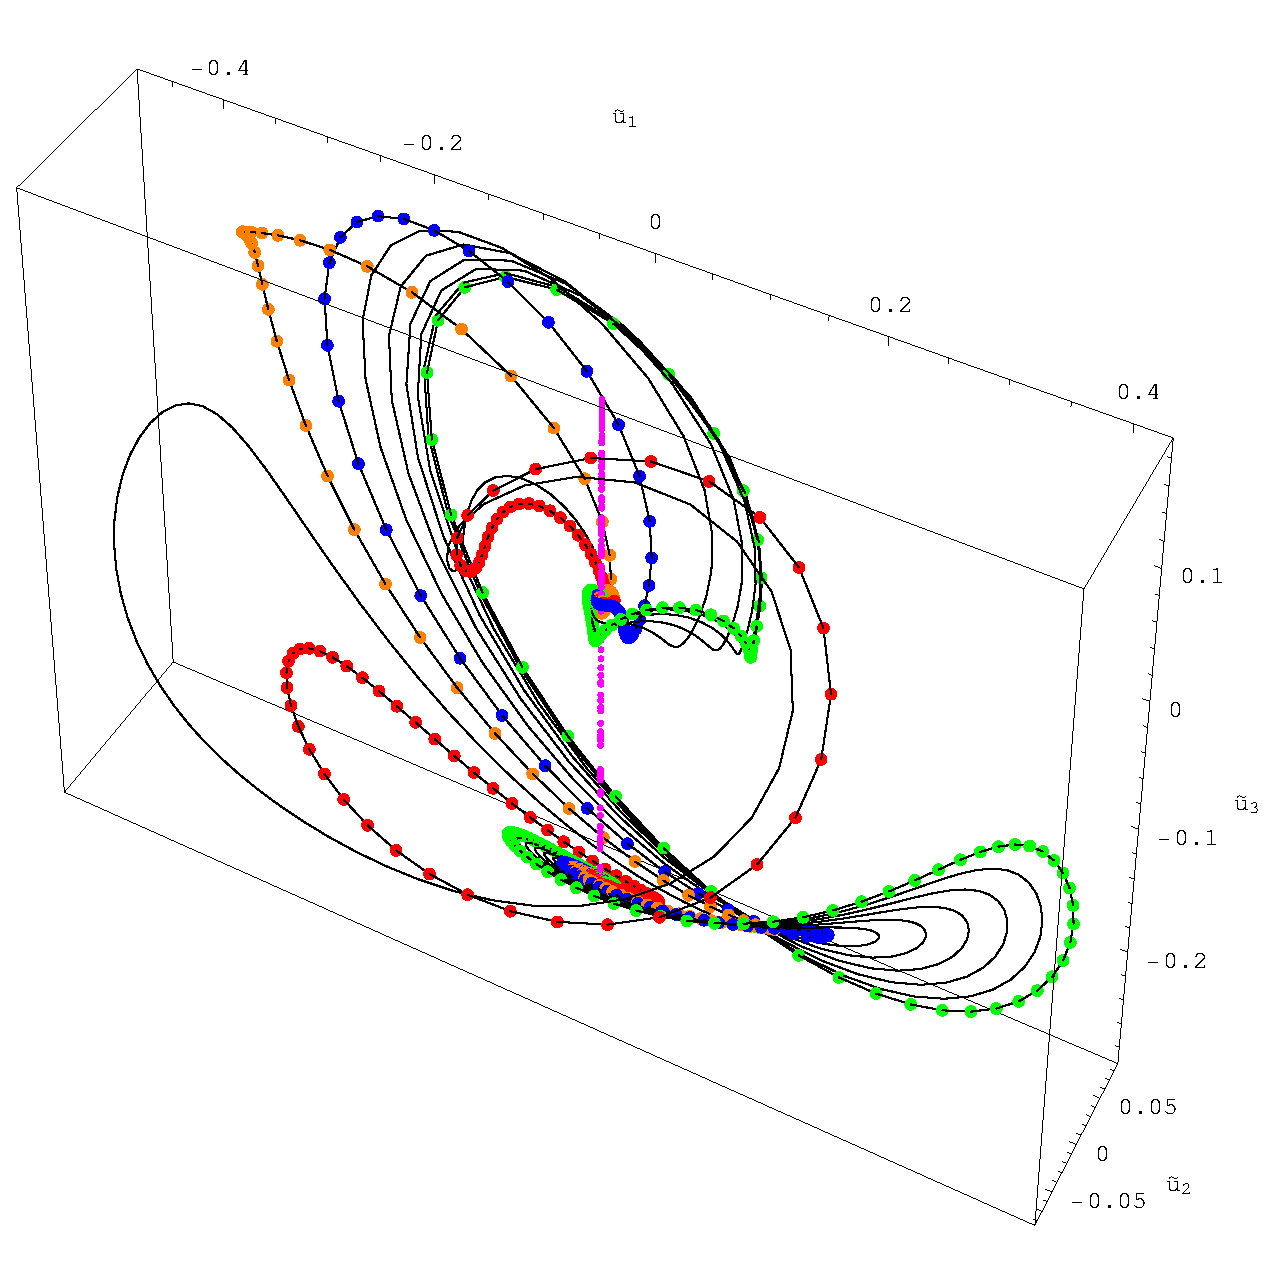
\includegraphics[width=5.0cm]{figs/L22-2w-UnsMan.eps}
\hspace{0.1in}
(b) \includegraphics[width=5.0cm]{figs/L22-2w-UnsMan-BlowUp.eps}
% (b) \includegraphics[width=4.0cm]{figs/L22-2w-R.eps}
\\
(c) \includegraphics[width=5.0cm]{figs/L22-2w-3w-UnsMan.eps}
% (c) \includegraphics[width=4.0cm]{figs/L22-2w-G.eps}
\hspace{0.1in}
(d)  \includegraphics[width=5.0cm]{figs/L22-2w-3w-detail.eps}
% (d) \includegraphics[width=4.0cm]{figs/L22-2w-B.eps}
\caption{
 Trajectories with initial conditions on the unstable subspace of
 the \nameit 2 {\eqva}.
 (a) The coordinates $\tilde{u}_1$ and $\tilde{u}_2$ are along the directions defining the unstable subspace
 and $\tilde{u}_3$  is along the real part of the eigenvector,
 corresponding to the eigenvalue $-0.271122+ i\, 0.356307$. The purple points represent the continous family
 of
\nameit 2 \eqva.
% Green curve belongs to \reffig{f:rpo55}(b) % rpo22-55-4-cm.eps
% rather than to  \reffig{f:rpo55}(a), % rpoEq22-55-4.eps?
(b) blowup of ``homoclinic'' descent of the unstable manifold
back into {\nameit}-2 {\eqv}, shifted by
$L/4 =5.5$.
(c) blowup of ``heteroclinc'' connection from
{\nameit}2 \eqv\ to {\nameit}3 \eqv\, with shift
$L(1/3-1/4) = L/12 = 1.83$ (? check)
to the neighborhood of the point near which the
unstable manifold of the
\nameit 2 \eqv\ splits. The blue points
represent the
\nameit 3 {\eqv} family.
The descent is along the eigenvector of $\Lyap_4= 0.413$ (checked by ES),
and spliting
occurs along one of the
$\Lyap_1=\Lyap_2=0.0933$
unstable directions of the \nameit 2 {\eqv} (checked by ES).
d) same as (c), closer to the \nameit 3 {\eqv}. The eigendirections corresponding to $\Lyap_1$
and $\Lyap_4$ are shown in purple.
}
\label{f:neighborhood2w}
\end{figure}
%%%%%%%%%%%%%%%%%%%%%%%%%%%%%%%%%%%%%%%%%%%%%%%%%%%%%%%%%%%%%%%%%%


\subsection{\Reqva}

In addition to the \eqva\ , the \KS\ system has \reqv\ solutions
(also called traveling or rotating waves in the literature).
They are characterized by a fixed function profile, $u(x)$,
moving with constant speed $c$, i.e.
\[ u(x+ct,t) = u(x, 0)\,,\quad t \in \mathbb{R}\,.\]
Because of the reflection symmetry, the \reqva\ come in pairs
related by the transformation: $u(x) \to -u(-x)$, $c \to -c$.
In Fourier space the \reqva\ are defined by the condition
\[ a_k(t)\mathrm{e}^{-iq_kct} = a_k(0)\,.\]
Differentiating this condition with respect to time, we obtain
equation for the \reqv\
\[ f_k(a) - i q_k c a_k = 0 \]
which needs to be solved for $a_k$ and $c$.

Consistent with the bifurcation diagram of Greene and Kim,
we find two \reqva\ with speeds $c = 0.737$ and $0.350$.
The profiles of the two \reqva\ and their time evolution
with eventual fall into the chaotic attractor are
shown in Figure~\ref{f:ks22tw}.


\underline{1-\reqv\  (traveling wave).}
% Ruslan L Davidchack,  10 Jul 2006
There is a pair of \reqva\
${\nameit}1L$,
${\nameit}1R$
(traveling waves), dual under the
$u(x) \to -u(-x)$ symmetry. They are
determined numerically by
adiabatic continuation from a smaller system size
$L~\approx 12$,
where they are stable, to $L=22$
where their velocity is atypically large, $c=0.737$,

Their exponents are:
\\
$\Lyap_i \pm \theta_i =
(
\\
  0.1156222 \pm 0.817289,   \\
  0.033663 \pm 0.418909,    \\
 0.0                    ,   \\
 -0.245729                    , \\
 -0.321321 \pm 0.98126,
\cdots
)$

The pair of \reqva\
${\nameit}2L$,
${\nameit}2R$
exists for larger system sizes, but does not continue
adiabatically\rf{KNSks90} down to $L=22$.


\subsection{\Eqva, $L$ and $c$}

%%%%%%%%%%%%%%%%%%%%%%%%%%%%%%%%%%%%%%%%%%%%%%%%%%%%%%%%%%%%%%%%
\begin{figure}[t]
    % \vspace*{-5pt}
\centering
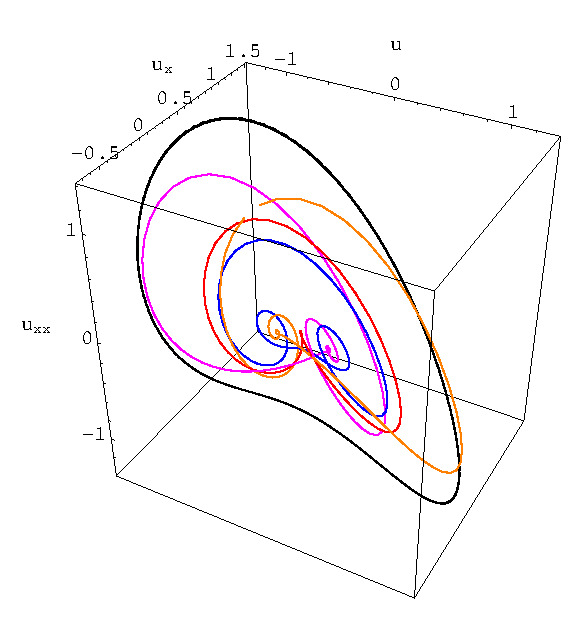
\includegraphics[width=0.6\textwidth]{figs/equilSpatial.eps}
    % \vspace*{-5pt}
\caption{
    {\small
$(u,u_x,u_{xx})$ representation
of $\EQV{1}$ (blue), $\EQV{2}$ (red), $\EQV{3}$ (black) \eqva\ and $\REQV{+}{1}$ (purple), $\REQV{-}{1}$ (orange) \reqva.
$\tildeL=3.5014$, $N=64$ complex modes truncation.
        } %end \small
        }
\label{f:eqvSpatial}
    % \vspace*{-5pt}
\end{figure}
%%%%%%%%%%%%%%%%%%%%%%%%%%%%%%%%%%%%%%%%%%%%%%%%%%%%%%%%%%%%%%%%%%

\PC{
 add the left/right $\REQV{\pm}{1}$ pair to \reffig{f:eqvSpatial}
    }
The $u=0$  \eqv\ $\EQV{0}$ is a point at the origin
in \reffig{f:eqvSpatial}.
At
each integer value of $\tildeL$ the origin spews out a Hopf cycle. That
might help us prove that we have all equilibria for $L=22$.

Each of these \eqva\ has a different value of the $c$ integration
constant.

Plot also the two \eqva\ of \eqva\ points, their
real eigenvectors and their complex eigenplanes. All equilibria presumably
wind around these, and as box size $L$ changes, they form continuous
families with smoothly changing $c$. One can check that by
changing $L$ a bit and using the previous equilibrium to find the next
one.

What does the complex eigenplane continuation does for these
equilibria - does it produce nice heteroclinic connections, or is it
wierder? We know there is an analytic formula for a heteroclinic
connection (see \refref{Lan:Thesis}). % Lan's thesis).

The real motivation for all this is that if we understand \eqva\ as
$L \to \infty$ we might have an entry into $L = \infty$ periodic orbit
theory of KS.

%%%%%%%%%%%%%%%%%%%%%%%%%%%%%%%%%%%%%%%%%%%%%%%%%%%%%%%%%%%%%%%%
\begin{figure}[h]
\centering
(a) \includegraphics[width=5.0cm]{figs/1wSteadyE.eps}
\hspace{0.1in}
(b) \includegraphics[width=5.0cm]{figs/1wSteadyP.eps}
\caption{
\small{
(a) $\EQV{1}$ in $(u,u_x,u_{xx})$ representation along with the eigenvectors of the equilibrium
point $(\sqrt{c},0,0)$. The blue line represents the unstable eigen-direction.
(b) $\EQV{1}$ projected along the above eigenvectors. $\tildeL=3.5014$, $N=64$ complex modes truncation.
}
}
\label{f:1wSteady}
\end{figure}

\reftab{tab:L22cminus} lists the stability eigenvalues
$\eigExp[1]^-,\eigRe[2]^-\pm\eigIm[2]^-$
of equilibrium point $c_{-}=(-\sqrt{c},0,0)$
of \label{eq:3dks} for $c$ corresponding to each on of $\EQV{1},\EQV{2}$ and $\EQV{3}$ \eqva.
The period of spiraling $T_{-}=2\pi/\theta^-_2$, expansion
rate in the complex plane of spiraling
$\ExpaEig_r\approx\exp(\eigRe[2]^- T_-)$ and contraction
rate along the stable eigendirection
$\ExpaEig_1\approx\exp(\eigRe[1]^- T_-)$ are also listed.

\begin{table}[h!]
% use packages: array
    \begin{tabular}{l|rrrrrr}
                & $E$   &$\eigExp[1]^-$ & $\eigRe[2]^-\pm\eigIm[2]^-$   & $T_m$ & $\ExpaEig_r$  & $\ExpaEig_1$  \\ \hline
        $\EQV{1}\ $ &\ 0.13 &\ -0.55    &\ $0.28\pm1.11i$       &\ 5.67     &\ 4.79     &\ 0.04 \\ \hline
        $\EQV{2}\ $     &\ 0.22 &\ -0.66    &\ $0.33\pm1.15i$       &\ 5.47     &\ 5.99     &\ 0.03 \\ \hline
        $\EQV{3}\ $     &\ 0.79 &\ -0.94    &\ $0.47\pm1.29i$       &\ 4.87     &\ 9.92     &\ 0.01
    \end{tabular}
    \caption{}
    \label{tab:L22cminus}
\end{table}


%%%%%%%%%%%%%%%%%%%%%%%%%%%%%%%%%%%%%%%%%%%%%%%%%%%%%%%%%%%%%%%%%%

% summary.tex
% $Author$ $Date$

\section{Summary}
\label{sect:rpo-sum}

We have presented a detailed investigation
of the geometry of the
{\KS} \statesp\ for $L=22$ system size, with emphasis on the role of
low-dimensional unstable manifolds of \eqva,
 and the connections between \eqva\ in organizing the flow.
A large number of unstable \rpo s and \po s has been determined
numerically.
Many of these \rpo s
\PCedit{appear} organized by the unstable manifold of $\EQV{2}$, closely
following the homoclinic loop formed between $\EQV{2}$ and $\Shift_{1/4}\EQV{2}$.


At first glance, turbulent dynamics visualized in the \statesp\ might appear
hopelessly complex, but under a detailed examination it is
much less so than feared: it is
pieced together from low dimensional 
local unstable manifolds connected by fast transient interludes.
{\KS} (and \pCf, see \refref{GHCW07})  \eqva, \reqva, \po s and
\rpo s embody Hopf's vision:
a repertoire of recurrent spatio-temporal
patterns explored by turbulent dynamics.
\PC{must expand this, emphasize novelty, especially
        of the \statesp\ visualization. See \refref{GHCW07}
        for inspiration.
        }


The key new feature of the full, periodic domain
KS, with its continuous translational symmetry,
are the attendant continuous families of
\reqva\ (traveling waves) and \rpo s.
\Rpo s, in particular, will require rethinking dynamical systems
approach to constructing symbolic dynamics.




\PC{
The real motivation for all this is that if we understand \eqva\ as
$L \to \infty$ we might have an entry into $L = \infty$ periodic orbit
theory of KS.
   }


% ackn.tex
% $Author$ $Date$

We thank Y.~Lan for determining
the $L=22$ \EQV{1}~\eqv.


\appendix

% fourierRLD.tex
% $Author$ $Date$

\section{Solving \KSe\ numerically}
\label{sec:fourierRLD}
% Predrag               jun 20 2006


The \KSe\ in terms of Fourier modes:
\beq
  \hat{u}_k = {\cal F}[u]_k = \frac{1}{L}\int_0^L u(x,t) e^{-i q_kx}dx\,,
  \qquad u(x,t) = {\cal F}^{-1}[\hat{u}] = \sum_{k\in{\mathbb Z}} \hat{u}_k e^{i q_k x}
\eeq
 is given by
\beq
  \dot{\hat{u}}_k = (q_k^2-q_k^4) \hat{u}_k -
  \frac{i q_k}{2}{\cal F}[({\cal F}^{-1}[\hat{u}])^2]_k\,.
\eeq
Since $u$ is real, the Fourier modes are related by $\hat{u}_{-k} =
\hat{u}^\ast_k$.

The above system is truncated as follows: The Fourier transform
${\cal F}$ is replaced by its discrete equivalent
\beq
  a_k = {\cal F}_N[u]_k = \sum_{n = 0}^{N-1} u(x_n)
  e^{-i q_k x_n}\,,\qquad u(x_n) = {\cal F}_N^{-1}[a]_n
  = \frac{1}{N}\sum_{k = 0}^{N-1} a_k e^{i q_k x_n}\,,
\eeq
where $x_n = 2\pi\tildeL/N$ and $a_{N-k} = a^\ast_k$.  Since $a_0
= 0$ due to galilean invariance and setting $a_{N/2} = 0$ (assuming
$N$ is even), the number of independent variables in the truncated
system is $N-2$.  The truncated system looks as follows:
\beq
  \dot{a}_k = \pVeloc_k(a) = [q_k^2-q_k^4]a_k -
  \frac{i q_k}{2}{\cal F}_N[({\cal F}_N^{-1}[a])^2]_k\,.
\ee{eq:KS}

where $k = 1,\ldots,N/2-1$.  Note that, since $a_k \in \mathbb{C}$,
\refeq{eq:KS} represents a system or ordinary differential equations in
${\mathbb R}^{N-2}$.
%, although in the Fourier transform we need
%to use $a_k$ over the full range of $k$ values from 0 to $N-1$.
The discrete Fourier transform ${\cal F}_N$ can be computed by FFT.
In Fortran and C, the FFTW library \refref{FFTW05} can be used.
% In Matlab, it is more convenient to use complex
% variables for $a_k$.  Note that Matlab function {\tt fft} is, in
% fact, the inverse Fourier Transform.

In order to find the Jacobian of the solution, or compute Lyapunov
exponents of the \KSe , one needs to solve the equation for a
displacement vector $b$ in the tangent space: \beq
  \dot{b} = \frac{\partial \pVeloc(a)}{\partial a} b\,.
\eeq
Since ${\cal F}_N$ is a linear operator, it is easy to show that
\beq
  \dot{b_k} = [q_k^2-q_k^4]b_k -
  iq_k{\cal F}_N[{\cal F}_N^{-1}[a]\cdot
  {\cal F}_N^{-1}[b]]\,,
\ee{eq:KStan}
where the dot indicates componentwise product of two vectors, \ie,
$a\cdot b = \diag(a)\,b = \diag(b)\,a$.  This
equation needs to be solved simultaneously with \refeq{eq:KS}.

When evaluating the Jacobian of the KS flow map, $J(a,t) = \partial
f^t(a)/\partial a$, the partial derivatives need to be evaluated
separately with respect to the real and imaginary parts of the
components of complex-valued vector $a$.  Therefore, the initial
conditions for \refeq{eq:KStan} that yield the partial derivative of
$f^t(a)$ with respect to Re $a_k$ and Im $a_k$, are $b_j(0) = 1 +
0i$ and $b_j(0) = 0 + 1i$, respectively, for $j = k$ and $b_j(0) =
0$ otherwise.

% lmderRLD.tex
% $Author$ $Date$

\section{Levenberg--Marquardt searches for \rpo s}
\label{sec:lmderRLD}

To find \rpo s of the \KSe , we use multiple shooting and
the Levenberg--Marquardt (LM) algorithm implemented in the routine
{\tt lmder} from the MINPACK software package\rf{minpack}.
% or function {\tt fsolve} in Matlab.

In order to find periodic orbits, a system of nonlinear
algebraic equations needs to be solved.  For flows, this
system is underdetermined, so, traditionally, it is augmented with
a constraint that restricts the search space to be transversal to the
flow (otherwise, most of the popular solvers of systems of nonlinear
algebraic equations, e.g. those based on Newton's method, cannot be used).
When detecting \rpo s, more constraints are added for each of the continuous
symmetries present in their definition.  For example, when detecting
relative periodic orbits in the complex Ginzburg�Landau equation (CGLE),
L{\'o}pez {\etal}\rf{lop05rel} introduce three additional constraints.

Our approach differs from those used previously in that we do not
introduce the constraints.  Note that, being an optimization solver,
the LM algorithm has no problem with solving an underdetermined systems of
equations, and, even though {\tt lmder} explicitly restricts the
number of equations to be not smaller than the number of variables,
the additional equations can be set identically equal to
zero\rf{Crofts07thesis}.  In fact, there is numerical evidence
that, when implemented with additional constraints, the
solver usually takes more steps to converge from the same seed,
or fails to converge at all\rf{Crofts07thesis}.

Below we give a detailed description of the algorithm and the
search strategy which we have used to find a large number
of \rpo s (RPOs) defined in \refeq{KSrpos} and pre-periodic orbits (PPOs)
defined in \refeq{KSpos}.

When searching for RPOs of the truncated \KSe\
(see \refeq{eq:KS}), we need to solve the system of $N-2$ equations
\beq
  {\bf g}(\shift)f^\period{}(a) - a = 0\,,
\ee{eq:system}
with $N$ unknowns $(a, \period{}, \shift)$, where $f^t$
is the flow map of the \KSe.  In the case of PPOs, the system has
the form
\beq
  -{\bf g}(-\shift)[f^\period{}(a)]^\ast - a = 0\,,
\ee{eq:systemppos}
(see \refeq{KSposFour}).

We have tried two different implementations of the multiple shooting.
The emphasis was on the simplicity of the implementations, so, even
though both implementations worked equally well, each of them had
its own minor drawbacks.

In the first implementation, we fix the total number of steps within
each shooting stage and change the numerical integrator step size
$h$ in order to adjust the total integration time to a desired value
$\period{}$.

Let $(\hat{a}, \hat{\period{}}, \hat{\shift})$ be the starting guess for a \rpo\
obtained through a close return within a chaotic attractor (see below).
We require that the initial integration step size
does not exceed $h_0$, so we round off the
number of integration steps to $n = \lceil \hat{\period{}}/h_0\rceil$, where
$\lceil x \rceil$ denotes the nearest integer larger than $x$.

The integration step size is equal to $h = \period{}/n$. With the
number of shooting stages equal to $m$, the system in
\refeq{eq:system} is rewritten as follows
\begin{eqnarray}\label{eq:MultShoot}
 F^{(1)}&\!=\!& f^\tau(a^{(1)}) - a^{(2)} = 0\,,\nonumber\\
 F^{(2)}&\!=\!& f^\tau(a^{(2)}) - a^{(3)} = 0\,,\nonumber\\
 && \cdots \\
 F^{(m-1)}&\!=\!& f^\tau(a^{(m-1)}) - a^{(m)} = 0\,,\nonumber\\
 F^{(m)}&\!=\!& {\bf g}(\shift)f^{\tau'}(a^{(m)}) - a^{(1)} = 0\,,\nonumber
\end{eqnarray}
where $\tau = \lfloor n/m \rfloor h$ ($\lfloor x \rfloor$ is the nearest
integer smaller than $x$),
$\tau' = nh - (m-1)\tau$, and $a^{(j)} = f^{(j-1)\tau}(a)$, 
$j = 1, \ldots , m$.  For the detection of PPOs, the last equation
in \refeq{eq:MultShoot} should be replaced with
\[
 F^{(m)} = -{\bf g}(-\shift)[f^{\tau'}(a^{(m)})]^\ast - a^{(1)} = 0\,.
\]
With the Jacobian matrix of \refeq{eq:MultShoot} written as
\beq
  J = \left(\begin{array}{ccc}\!\!
   \displaystyle \frac{\partial F^{(j)}}{\partial a^{(k)}} &
   \displaystyle \frac{\partial F^{(j)}}{\partial \period{}} &
   \displaystyle \frac{\partial F^{(j)}}{\partial \shift}\!\!
  \end{array}\right),\quad j,k = 1,\ldots,m\,,
\eeq
the partial derivatives with respect to $a^{(k)}$ can be calculated
using the solution of \refeq{eq:KStan} as described in
Appendix~\ref{sec:stability}.  The partial derivatives
with respect to $T$ are given by
\beq
  \frac{\partial F^{(j)}}{\partial \period{}} =
  \left\{\begin{array}{ll}
    \frac{\partial f^\tau(a^{(j)})}{\partial \tau}
    \frac{\partial \tau}{\partial T} = v(f^\tau(a^{(j)}))
    \lfloor n/m \rfloor/n\,, & j = 1,\ldots, m-1\\[.5ex]
    {\bf g}(\shift) v(f^{\tau'}(a^{(j)}))
    (1 - \frac{m-1}{n} \lfloor n/m \rfloor ), & j = m\,.
  \end{array}\right.
\eeq
Note that, even though $\partial f^t(a) /\partial t = v(f^t(a))$,
it should not be evaluated using equation for the vector field.
The reason is that, since the flow $f^t$ is approximated by a
numerical solution, the derivative of the numerical solution with
respect to the step size $h$ may differ from the vector field $v$,
especially for larger step sizes.  We evaluate the derivative by
a forward difference using numerical integration with step sizes
$h$ and $h + \delta$:
\beq
  \frac{\partial f^{jh}(a)}{\partial t} = \frac{1}{j\delta}
  \left[f^{j(h+\delta)}(a) - f^{jh}(a)\right],\quad j \in
  {\mathbb Z}^{+}
\eeq with $t = jh$ and $\delta = 10^{-7}$ for double precision
calculations. Partial derivatives $\partial F^{(j)}/\partial \shift$
are all equal to zero except for $j = m$, where it is given by
\beq
  \frac{\partial F^{(m)}}{\partial \shift} =
  \frac{d{\bf g}}{d\shift}f^{\tau'}(a^{(m)}) =
  \diag(i q_k e^{i q_k\, \shift} )f^{\tau'}(a^{(m)})\,.
\eeq

This Jacobian is supplied to {\tt lmder}
augmented with two rows of zeros corresponding to the two identical
zeros augmenting \refeq{eq:MultShoot} in order to make the number of
equations formally equal to the number of variables,
as discussed above.

In the second implementation, we keep $h$ and $\tau$ fixed and vary
only $\tau' = \period{} - (m-1)\tau$.  In this case, we need to be
able to determine the numerical solution of \KSe\ not only at times
$t_j = jh, j = 1, 2, \ldots$, but at any intermediate time as well.
We do this by a cubic polynomial interpolation through points
$f^{t_j}(a)$ and $f^{t_{j+1}}(a)$ with slopes $v(f^{t_j}(a))$ and
$v(f^{t_{j+1}}(a))$.  The difference from the first implementation
is that partial derivatives $\partial F^{(j)}/\partial \period{}$
are zero for all $j = 1,\ldots,m-1$, except for
\beq
  \frac{\partial F^{(m)}}{\partial \period{}} =
  {\bf g}(\shift)v(f^{\tau'}(a^{(m)}))\,.
\eeq
which, for consistency, needs to be evaluated from the cubic
polynomial, not from the flow equation evaluated
at $f^{\tau'}(a^{(m)})$.

For detecting \rpo s of the \KSe\ with $L = 22$, we used
$N = 32$, $h = 0.25$ (or $h_0 = 0.25$ within the first implementation),
and the number of shooting stages such that $\tau \approx 40.0$.
While both implementations were equally successful in detecting
periodic orbits of \KSe , we found the second implementation more
convenient.

The following search strategy was adopted: The search for \rpo s with
$\period{} \in [10, 200]$ was conducted within a rectangular region
containing the chaotic attractor.  To generate a seed, a random point was
selected within the region and the flow \refeq{eq:KS} was
integrated for a transient time $t = 40$, sufficient for an orbit
to settle on the attractor at some point $\hat{a}$.  This point was taken
to be the seed location.  In order to find orbits with different
periods, the time interval $[10, 200]$ was subdivided into windows
of length 10, i.e. $[t_\mathrm{min}, t_\mathrm{max}]$, where
$t_\mathrm{min} = 10j$ and $t_\mathrm{max} = 10(j+1)$, with
$j = 1, 2, \ldots, 19$.  To determine the seed time
$\hat{\period{}}$ and shift $\hat{\shift}$, we located an
approximate global minimum of $\| \pm{\bf g}(\pm\shift)f^t(a) - a \|$ as
a function of $t \in [t_\mathrm{min}, t_\mathrm{max}]$ and
$\shift \in (-L/2, L/2]$.  We did this simply by finding the minimum
value of the function on a grid of points with resolution $h$
in time and $L/50$ in $\shift$.

Once a \rpo\ is found, its existence in the \KS\ PDE is verified
 numerical approximation improved by increasing the number of
Fourier modes ($N = 64$) and reducing the step size ($h = 0.1$).
    \edit{
Among the thousands of orbits
computed in this study only two failed this higher-resolution test.
    }

% newton.tex
%
% Predrag			jun 20 2006
% Vaggelis			may 20 2006
% $Author$ $Date$


% \section{Newton's method for determining \reqva}
% 
%  Our task is to find \reqva\ solutions of \refeq{eq:KS}.
% Although one can easilly see that this problem can be reduced to that of
%  finding periodic orbits of a 4-dimensional ODE, here we prefer to consider our system in phase space and search for solutions of
%  \beq
% 	\dot{b}_k=\dot{c}_k=0\,,
%  \eeq
%  for every $k$. The reason to do this is just getting experience before pursuing the more difficult task of locating POs and RPOs. 
%  Expanding $\dot{b}_k(a)$ and $\dot{c}_k(a)$ around our initial guess $a_o$ and demanding that they satisfy the equilibrium 
%  condition, we get
%  \bea
% 	\dot{b}_k(a) & = & \dot{b}_k(a_o)+\left.\frac{\partial \dot{b}_k}{\partial b_j}\right|_{a_o}\delta b_j + \left.\frac{\partial \dot{b}_k}{\partial c_j}\right|_{a_o}\delta c_j = 0 \continue
% 	\dot{c}_k(a) & = & \dot{c}_k(a_o)+\left.\frac{\partial \dot{c}_k}{\partial b_j}\right|_{a_o}\delta b_j + \left.\frac{\partial \dot{c}_k}{\partial c_j}\right|_{a_o}\delta c_j = 0
%  \eea
%  or in matrix form
%  \beq
%     \left( \begin{array}{cc}
%         \frac{\partial \dot{b}}{\partial b} & \frac{\partial \dot{b}}{\partial c} \\
%         \frac{\partial \dot{c}}{\partial b}	& \frac{\partial \dot{c}}{\partial c}
%      \end{array}
%      \right)_{a_o}
%      \left(\begin{array}{c}
%        \delta b  \\
%        \delta c
%      \end{array}\right)
%      =
%      \left(\begin{array}{c}
%        -\dot{b}(a_o) \\
%        -\dot{c}(a_o)
%      \end{array}\right)\,,
%      \label{eq:NewtonEquil}
% \eeq
% where $\partial{\dot{b}} / \partial{b}$ \etc are $d \times d$ submatrices. Solving this
% system of equations for the corrections $\delta b$ and  $\delta c$ and using the refined solution
% as an initial guess yields  an approximation to the solution of the system.
%  


\subsection{Implementing Newton's method  for RPOs}
\label{sec:NewtRPOs}

The relative periodic condition
\beq
	u(x+d,t+T)=u(x,t) \,
\eeq
translates in Fourier space into
\beq	
	\sum_{k=-\infty}^{+\infty} a_k (t+T) e^{ i k (x+d) / \tildeL} 
		= \sum_{k=-\infty}^{+\infty} a_k (t) e^{ i k x / \tildeL} \,
\eeq
or
\beq
	e^{ik\, d /\tildeL}a_k(t+T)=a_k(t) \,,\ \forall k \in \mathds{Z}\ \ \ \mathrm{(no\ summation)}.
	\label{eq:RPOcondition}
\eeq
We see that a relative periodic orbit returns after time $T$ to a point in 
phase space with components $a_k(t+T)$ rotated in the complex plane by an 
angle $-k\, d /\tildeL$ with respect to $a_k(t)$. In matrix notation, we write \refeq{eq:RPOcondition} as
\beq
	\mathbf{g}(d)  a(t+T)=a(t)\,,
	\label{eq:RPO}
\eeq
where we have defined
\beq
	\mathbf{g}(d) \equiv Diag[e^{ik\, d/\tildeL}]\,.
\eeq
%We notice that $R(\kappa)$ is not a rotation operator..

% Consider an initial guess $a'$ for a point on a relative periodic orbit and assume that it lies on
% a \Poincare section $\mathcal{P}$ at $t=0$. Suppose that $\mathcal{P}$ is a hyperplane in
% $\mathds{R}^{2d}$. The flow $f^t$ defined by \refeq{eq:Fcoef} transports 
% this point after time $T'$ into $a'(T')=f^{T'}(a')$. Suppose that this point is such that $R(\kappa')f^{T'}(a')$
% is a point on $\mathcal{P}$. Consider next a point $a$ lying on $\mathcal{P}$ and in the neighborhood of $a'$,
% thus satisfying
% \beq
% 	q \cdot (a'-a) = 0\,,
% 	\label{eq:cond a}
% \eeq
% with $q$ a vector normal to $\mathcal{P}$. Point $a$ will be finally identified with the improved 
% approximation of a point on the periodic orbit.
% The flow transports $a$ to $f^{T'}(a)$, but now $R(\kappa')f^{T'}(a)$ is not in general on $\mathcal{P}$.
% Moreover we would like to have the freedom to adjust the guesses for $T'$ and $\kappa'$ into new values
% $T=T'+\Delta T$ and $\kappa=\kappa'+\Delta \kappa$ to improve their accuracy. 
% Let as consider such slightly different values $T$ and $\kappa$ such that $R(\kappa)f^{T}(a)$ lies on 
% $\mathcal{P}$. Then we have the condition
% \beq
% 	q \cdot(R(\kappa')f^{T'}(a')-R(\kappa)f^{T}(a)) = 0\,.
% 	\label{eq:cond Rf(a)}
% \eeq 

Starting with an initial guess $a$ for a point on a \rpo\ we use Newton's method to find an improved approximation to the true solution $a^*$ of condition  \refeq{eq:RPO}:
\beq
	a^*=\mathbf{g}(d^*)  f^{T^*}(a^*)\,,
	\label{eq:RPOcond}
\eeq
with period $T^*$ and shift $d^*$. Let $T$ and $d$ be our guess period and shift, respectively. 
Taylor expanding $\mathbf{g}(d^*)  f^{T^*}(a^*)$ around $a$ to linear order in the small quantities 
$\delta a=a^*-a$, $\delta T=T^*-T$ and $\delta d=d^*-d$, we get
% \bea
% 	f^{T}(a)& \simeq & f^{T}(a')+\J^T(a') \Delta a \label{eq:fTaylorl1} \\ 
% 		& \simeq & f^{T'}(a') + v \Delta T + \J^{T'}(a') \Delta a \label{eq:fTaylorl2} \,, 
% \eea
% where $v$ is evaluated at $f^{T'}(a')$. Here $\J^t(x)$ is the Jacobian matrix, defined for a general flow through
% \beq
%    	J^t_{ij}(x_o)=\left.\frac{\partial x_i(t)}{\partial x_j}\right|_{x=x_0}\,.
% \eeq
% The Jacobian matrix is obtained by integrating the equation:
% \beq
%    	\dot{\mathbf{J}}^t=\mathbf{A J}^t \, ,
% 	\label{eq:Adef}
% \eeq
% subject to the initial condition:
% \beq
%    	\mathbf{J}^0=\mathbf{1} \, ,
% \eeq
% Here $\mathbf{A}$ is the matrix of variations defined as:
% \beq
% 	A_{kj}=\frac{\partial \dot{x}_k}{\partial x_j}\,.
% \eeq
% 
% In passing from \refeq{eq:fTaylorl1} to \refeq{eq:fTaylorl2} we have used the multiplicative 
% structure of the Jacobian, $\mathbf{J}^{T'+\delta T}(a')=\mathbf{J}^{\delta T}(f^{T'}(a'))\mathbf{J}^{T'}(a')$, 
% noticed that $\mathbf{J}^{\delta T}(f^{T'}(a'))=e^{\mathbf{A}\delta T}=\mathbf{1}+\mathbf{A}\delta T+\ldots$ 
% and dropped second order terms in the small quantities.
% 
% On the other hand, we have
% \bea
% 	R(\kappa'+\Delta\kappa) & = & R(\kappa')R(\Delta\kappa) \continue
% 				& \simeq & R(\kappa')(\mathbf{1}+iDiag[k]\Delta\kappa/\tildeL)\,.
% 	\label{eq:TaylorR}	
% \eea
% 
% Substituting \refeq{eq:fTaylorl2},\refeq{eq:TaylorR} into \refeq{eq:RPOcond} and keeping only first
% order terms in the small quantities, we get
% \beq
% 	a+\delta a \simeq \mathbf{g}(d)  f^{T}(a) + \mathbf{D[g]}(\mathbf{g}(d) f^{T}(a))\delta d
% 				+ \mathbf{g} (d)v(f^{T}(a)) \delta T + \mathbf{g}(d) \J^{T}(a) \delta a\,,
% \eeq
% or
\beq
	\left(\mathbf{1}-\mathbf{g}(d)\J^{T}(a)\right) \delta a - \mathbf{g}(d)v(f^{T}(a)) \delta T 
							- \mathbf{D[g]}(\mathbf{g}(d)f^{T}(a))\delta d  
					\,\simeq\, \mathbf{g}(d)f^{T}(a)-a\,,
	\label{eq:NewtonBasicCond}			
\eeq
where $D[g]_{kj}=\frac{ik}{\tildeL}\delta_{kj}$. The matrix $\mathbf{g}(d)\J^{T}(a)$ has two unit eigenvalues in 
the limit $a\rightarrow a^*$, one associated with the invariance along the direction of the flow and the other with the
translational invariance of the system. Thus \refeq{eq:NewtonBasicCond} needs to be augmented by two conditions to
eliminate the indeterminacy introduced by the (close to) zero eigenvalues of $\mathbf{1}-\mathbf{g}(d)\J^{T}(a)$. Following 
\refref{ViswanathPC06} we choose the conditions 
\bea
	v(a)\cdot\delta a & = & 0 \label{eq:NewtonAux1} \,\\
	(\mathbf{D[g]}a)\cdot \delta a & = & 0 \label{eq:NewtonAux2}\,.
\eea
The requirement imposed by \refeqs{eq:NewtonAux1}{eq:NewtonAux2}\ on the solution vector $\delta a$ of \refeq{eq:NewtonBasicCond} 
is that it vanishes along the directions of the flow and of infinitesimal translation of the initial condition.

Equations \refeq{eq:NewtonBasicCond} and \refeqs{eq:NewtonAux1}{eq:NewtonAux2}
can be compactly represented in a single matrix equation:
\beq
    \left( \begin{array}{ccc}
       \mathbf{1}-\mathbf{g}(d)\mathbf{J}^{T}(a) 	& -\mathbf{g}(d)v(f^{T}(a))	  & -\mathbf{D[g]}(\mathbf{g}(d)f^{T}(a))  \\
        v(a)^{\dagger}			& 0  	& 0 	\\
        (\mathbf{D[g]}a)^\dagger	& 0 	& 0 
     \end{array}
     \right)
     \left(\begin{array}{c}
       \delta a \\
       \delta T \\
       \delta d
     \end{array}\right)
     =
     \left(\begin{array}{c}
       \mathbf{g}(d)f^{T}(a)-a \\
       0     \\
       0
     \end{array}\right)\,.
     \label{eq:NewtonScheme}
\eeq
where $v^\dagger$ denotes the adjoint of $v$. 




\bibliography{../bibtex/siminos}


\end{document}
